\documentclass[tikz,border=2pt]{standalone}
\usetikzlibrary{positioning}
\usetikzlibrary{patterns}
\usetikzlibrary{arrows.meta}
\usetikzlibrary{calc}
\usepackage{amsmath}
\usepackage{amssymb}
\usepackage{mathrsfs}
\usepackage{graphicx}
\usepackage{tikz}
\usepackage{xcolor}
\newcommand{\R}{\mathbb R}
\newcommand{\C}{\mathbb C}
\newcommand{\Z}{\mathbb Z}
\newcommand{\N}{\mathbb N}
\newcommand{\T}{\mathbb T}
\newcommand{\E}{\mathbb E}
\newcommand{\PP}{\mathbb P}
\newcommand{\dd}{\,\mathrm d}
\newcommand{\one}{\mathbf 1}
\newcommand{\norm}[1]{\left\lVert#1\right\rVert}
\newcommand{\abs}[1]{\left\lvert#1\right\rvert}
\DeclareMathOperator{\supp}{supp}
\DeclareMathOperator{\dist}{dist}
\DeclareMathOperator{\diam}{diam}
\DeclareMathOperator{\tr}{tr}
\DeclareMathOperator{\diag}{diag}
\DeclareMathOperator{\rank}{rank}
\DeclareMathOperator{\Law}{Law}
\begin{document}
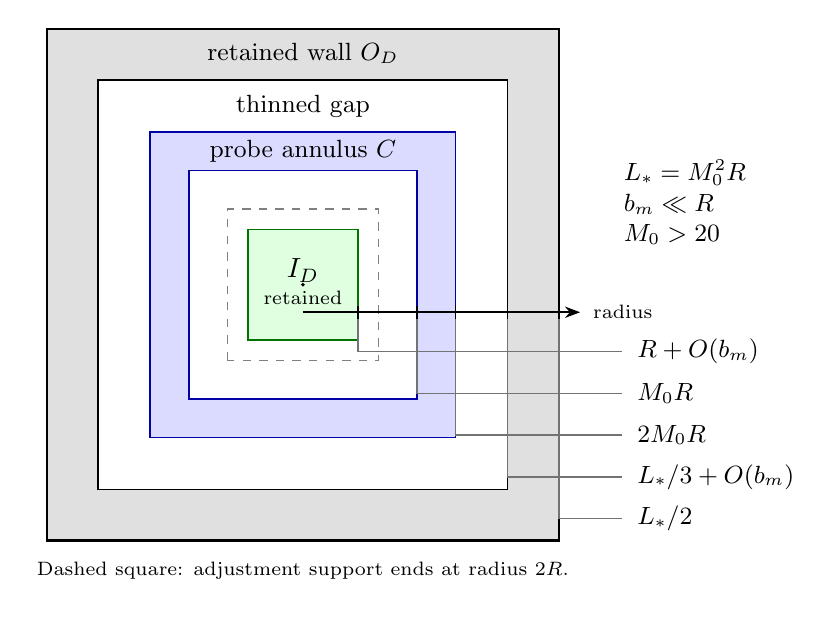
\begin{tikzpicture}[x=1cm,y=1cm,>=Stealth, line width=0.55pt]
  \fill[black!12,even odd rule]
    (-3.25,-3.25) rectangle (3.25,3.25)
    (-2.60,-2.60) rectangle (2.60,2.60);
  \fill[blue!14,even odd rule]
    (-1.94,-1.94) rectangle (1.94,1.94)
    (-1.45,-1.45) rectangle (1.45,1.45);
  \fill[green!12] (-0.70,-0.70) rectangle (0.70,0.70);
  \draw[thick] (-3.25,-3.25) rectangle (3.25,3.25);
  \draw (-2.60,-2.60) rectangle (2.60,2.60);
  \draw[blue!65!black] (-1.94,-1.94) rectangle (1.94,1.94);
  \draw[blue!65!black] (-1.45,-1.45) rectangle (1.45,1.45);
  \draw[green!45!black] (-0.70,-0.70) rectangle (0.70,0.70);
  \draw[dashed,black!50] (-0.96,-0.96) rectangle (0.96,0.96);
  \node at (0,0.18) {$I_D$};
  \node[font=\scriptsize] at (0,-0.16) {retained};
  \node[font=\small] at (0,2.27) {thinned gap};
  \node[font=\small] at (0,1.69) {probe annulus $C$};
  \node[font=\small] at (0,2.94) {retained wall $O_D$};
  \fill (0,0) circle (0.025);
  \draw[->] (0,-0.35) -- (3.52,-0.35);
  \node[anchor=west,font=\scriptsize] at (3.56,-0.35) {radius};
  \draw (0.70,-0.43) -- (0.70,-0.27);
  \draw (1.45,-0.43) -- (1.45,-0.27);
  \draw (1.94,-0.43) -- (1.94,-0.27);
  \draw (2.60,-0.43) -- (2.60,-0.27);
  \draw (3.25,-0.43) -- (3.25,-0.27);
  \draw[black!55] (0.70,-0.44) -- (0.70,-0.85) -- (4.05,-0.85);
  \draw[black!55] (1.45,-0.44) -- (1.45,-1.38) -- (4.05,-1.38);
  \draw[black!55] (1.94,-0.44) -- (1.94,-1.91) -- (4.05,-1.91);
  \draw[black!55] (2.60,-0.44) -- (2.60,-2.44) -- (4.05,-2.44);
  \draw[black!55] (3.25,-0.44) -- (3.25,-2.97) -- (4.05,-2.97);
  \node[anchor=west,font=\small] at (4.12,-0.85) {$R+O(b_m)$};
  \node[anchor=west,font=\small] at (4.12,-1.38) {$M_0R$};
  \node[anchor=west,font=\small] at (4.12,-1.91) {$2M_0R$};
  \node[anchor=west,font=\small] at (4.12,-2.44) {$L_*/3+O(b_m)$};
  \node[anchor=west,font=\small] at (4.12,-2.97) {$L_*/2$};
  \node[align=left,anchor=west,font=\small] at (3.95,1.05)
    {$L_*=M_0^2R$\\$b_m\ll R$\\$M_0>20$};
  \node[font=\scriptsize,align=center] at (0,-3.63)
    {Dashed square: adjustment support ends at radius $2R$.};
\end{tikzpicture}
\end{document}
